\begin{frame}{\insertsubsection}
  Cargo plugins

  \begin{itemize}
  \item cargo-asm
  \item cargo-call-stack
  \item cargo-clippy
  \item cargo-fmt
  \item cargo-fuzz
  \item cargo-geiger
  \item cargo-graph
  \item cargo-install-update
  \item cargo-llvm-ir
  \item cargo-profdata
  \item cargo-size
  \item many others!
  \end{itemize}

  \note {

    Для cargo можно устанавливать плагины.

    \begin{itemize}
    \item для показа CFG, DFG
    \item для автоматического форматирования всего проекта
    \item для автоматического фаззинга
    \item для нахождения неидиоматичного кода с последующим автоматическим
      исправлением
    \item для генерации промежуточного представления
    \item для профилирования
    \item ещё куча всего!
    \end{itemize}

  }

\end{frame}

\begin{frame}[fragile]{\insertsubsection}
  \begin{minted}[gobble = 4, frame = lines, linenos, breaklines, label =
    Sanitize code]{shell}
    $ RUSTFLAGS="-Z sanitizer=address" cargo test
    $ RUSTFLAGS="-Z sanitizer=leak" cargo test
    $ RUSTFLAGS="-Z sanitizer=memory" cargo test
    $ RUSTFLAGS="-Z sanitizer=thread" cargo test
  \end{minted}

  \note{

    Например, вот так просто вызываются санитайзеры для кода.

  }
\end{frame} 

\begin{frame}{Services}

  \begin{columns}
    \begin{column}{.4\textwidth}
      \begin{itemize}
      \item Rust documentation
      \item Crates.io --- all packages
      \item Docs.rs --- all documentation
      \item Rust book
      \end{itemize}
    \end{column}
    \begin{column}{.6\textwidth}
      \center%
      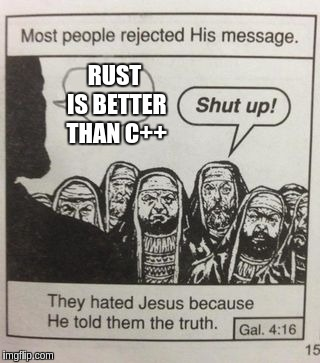
\includegraphics[height = .8\textheight]{rust_is_better.jpg}
    \end{column}
  \end{columns}

  \note {

    Как у любого уважающего себя языка, у Rust есть \textbf{online документация}
    по самому языку и по стандартной библиотеке.

    Также есть удобный \textbf{сайт со всеми пакетами}.

    А к нему есть официальный сайт с \textbf{автогенерируемой документацией по
      всем пакетам}. \textbf{И всё в одном стиле}!

    Есть уже \textbf{второе издание online книги по Rust}, также есть печатная
    версия. Советую ознакомиться. Кроме этой книги, есть ещё \textbf{пара
      официальных для более продвинутых}.

  }

\end{frame}
